\begin{figure}
    \centering
    \begin{minipage}{0.32\textwidth}
        \centering
        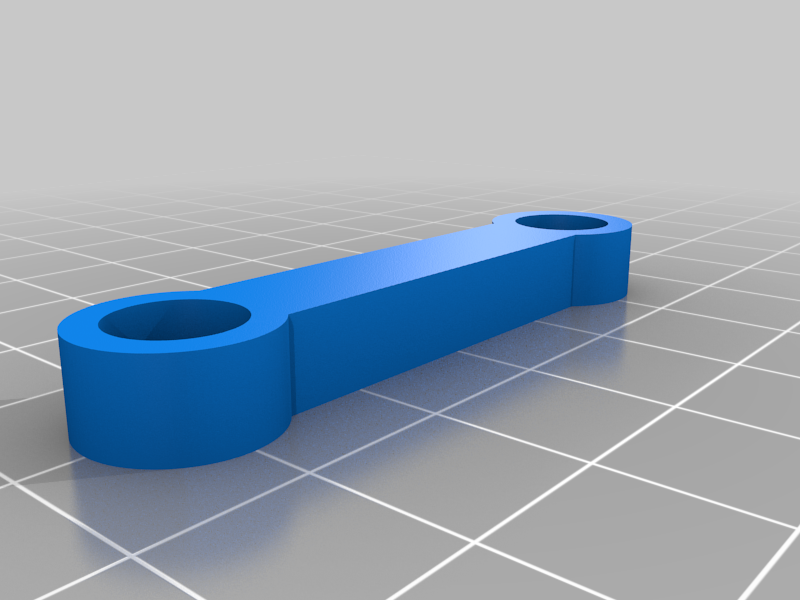
\includegraphics[width=\textwidth]{papers/geradlinig/figures/link_driver.png}
    \end{minipage}
    \hfill
    \begin{minipage}{0.32\textwidth}
        \centering
        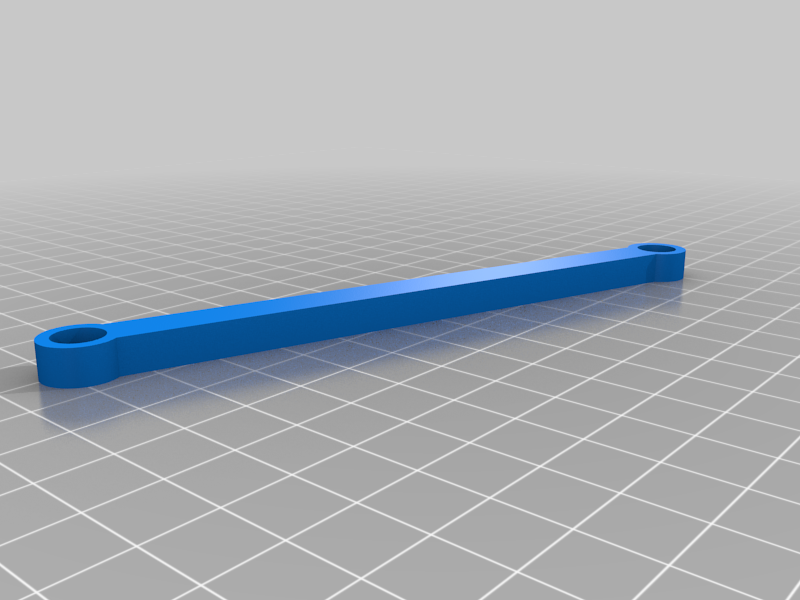
\includegraphics[width=\textwidth]{papers/geradlinig/figures/link_long_lower.png}
    \end{minipage}
    \hfill
    \begin{minipage}{0.32\textwidth}
        \centering
        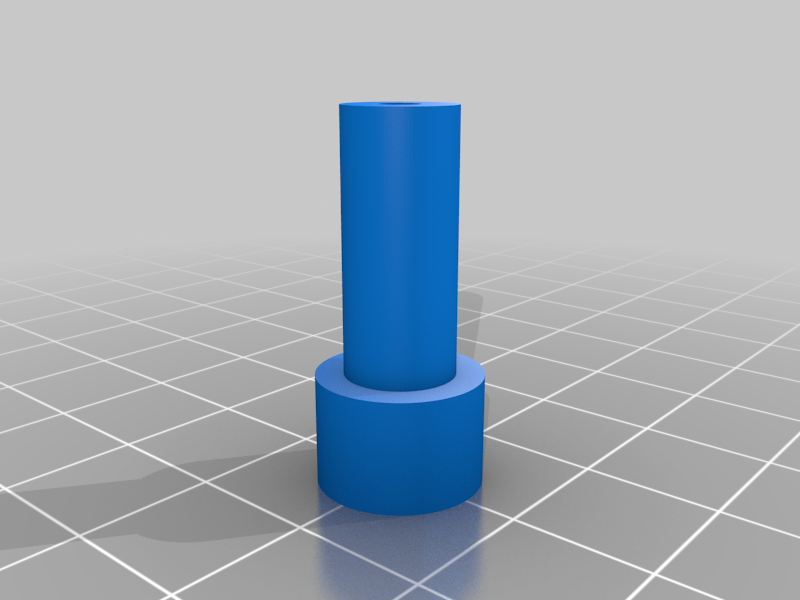
\includegraphics[width=\textwidth]{papers/geradlinig/figures/pin_lower.png}
    \end{minipage}
    \caption{Beispiele für Standardgelenke und Bolzen 
    für den 3D-Druck~\cite{thingiverse}.}
    \label{fig:3dprint_mech}
\end{figure}
